\chapter{Methodology}
To perform agile flight through cluttered and previously-unseen environments, we train a sensorimotor policy to predict receding-horizon \cite{receding_horizon}
trajectories from on-board sensor measurements and a reference trajectory. We assume that the reference trajectory is provided by a higher level planning algorithm \cite{global_planning} or the user. The reference is not necessarily
collision-free and only encodes the long-term goal of the platform. The
agent is responsible to fly in the direction dictated by the reference
while adapting its flight path to the environment.

\textbf{An agent’s observation $o$ consists of a depth image $d \in \R^{640*480}$,
an estimate of the platform velocity $v \in \R^3$ and attitude (expressed as
a rotation matrix) $q \in \R^9$ , and a desired flight direction $\omega \in \R^3$. }

The
policy output is a set of motion hypotheses which are represented as
receding-horizon \cite{receding_horizon} trajectories with the corresponding estimated risk of
collision. A model predictive controller then tracks the trajectory with
 the lowest collision probability and input cost. The controller is trained
using privileged learning.


\section{Training}
Training are performed entirely in simulation. This facilitates access to perfect 3D and state data for the
privileged expert. Flightmare simulator with the RotorS Gazebo plugin and Unity as a rendering engine is used to train and test the model. Both the training
and the testing environments are built by adding obstacles to the uneven
ground of an out-of-the-box Unity environment.

To enable zero-shot transfer to real environments, the sensorimotor agent is trained with depth images that have been
computed using Semi-Global Matching (SGM) \cite from a simulated
stereo camera pair \cite{stereoMatching}. 

\subsection{Method Overview}
As shown in figure \ref{fig:method-overview}, the offline planning algorithm computes a distribution of collision-free trajectories to follow a reference trajectory. The trajectories are computed with Metropolis-Hastings \cite{MH_hasting} sampling and are conditioned on complete 3D knowledge of the environment, which is represented by a point cloud. A sensorimotor agent is trained with imitation learning to predict the best three trajectories from the estimated depth, the drone’s velocity and attitude, and the desired direction that encodes the goal. The predictions are projected on the
space of polynomial trajectories and ranked according to their predicted collision cost $c_k$ . The trajectory with the lowest predicted cost is then
tracked with a model predictive controller. If multiple trajectories have similar predicted cost (within a 5 percent range of the minimum $c^* = min$ $c_k$ ),
the one with the smallest actuation cost is used.

\begin{figure}[!h]
	\centering
	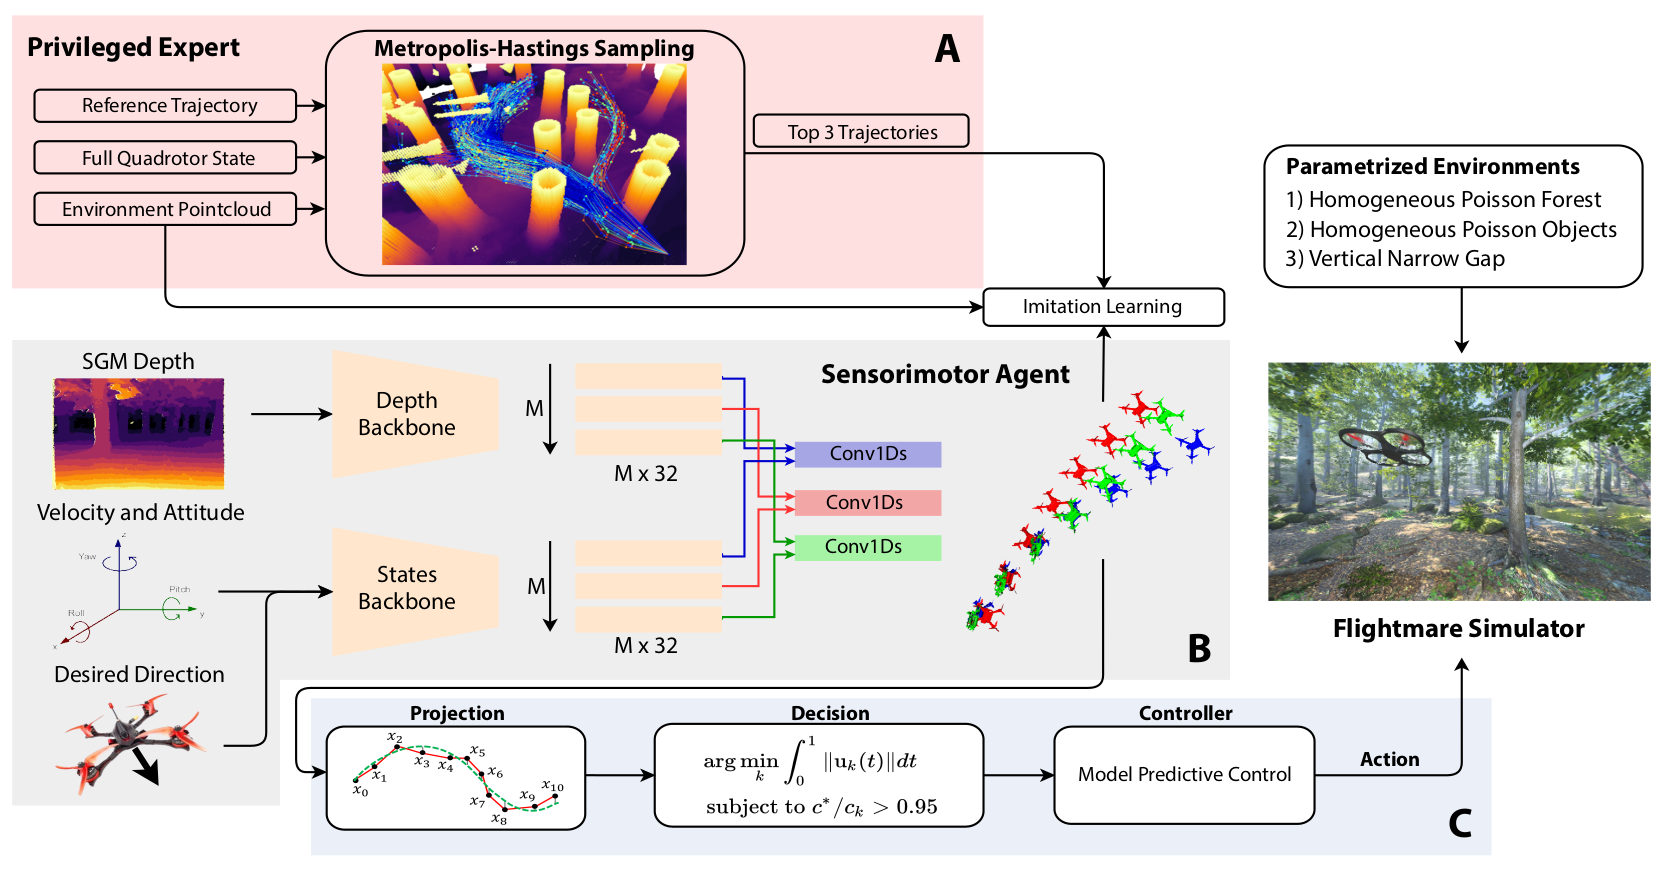
\includegraphics[width=\textwidth]{method-overview.png}
	\caption{Method Overview}
	\label{fig:method-overview}
	
\end{figure}

\section{The Privileged Expert}
Privileged expert is a sampling-based motion planning algorithm \cite{MH_hasting}.
The expert has perfect knowledge of the platform state and the environment (complete 3D map). The expert generates a set of collision-free trajectories $\tau$ representing the desired state of the quadrotor $x_{des} \in \R^13$ over the
next second, starting from the current state of the drone.

To do so, it samples from a probability distribution $P$ that encodes distance from obstacles and proximity to the reference trajectory. The distribution of collision-free trajectories $P(\tau | \tau_{ref}, C)$ is
conditioned on the reference trajectory $\tau_{ref}$ and the structure of the
environment in the form of a point cloud $C \in \R^{n*3}$ . According to $P$,
the probability of a trajectory $\tau$ is large if far from obstacles and close
to the reference $\tau_{ref}$ . The $P$ is defined as the following:
\begin{equation}
	P(\tau | \tau_{ref},C) = \frac{1}{Z} exp(-c(\tau, \tau_{ref},C)) \\
\end{equation}
Where $	Z = \int_{\tau} P(\tau | \tau_{ref},C)$ is the nomalization factor and $c(\tau, \tau_{ref},C) \in \R_+$ is a cost function indication proximity to the reference and distance from obstacles. The trajectory cost function is defined as 
\begin{equation}
	c(\tau, \tau_{ref},C) = \int_0^1 \lambda_c C_{collision}(\tau(t)) + \int_0^1 [\tau(t)-\tau_{ref}(t)]^T Q[\tau(t)-\tau_{ref}(t)]{dt}
	\label{eqn:collision}
\end{equation}
where $\lambda_c = 1000$, $Q$ is a positive semidefinite state cost matrix and $C_{collision}$ is a measure of the distance of the quadrotor to the points in $C$

We model the quadrotor as a sphere of radius $r_q$ and define the collision cost as a quadratic function of $d_c$ (distance between the quadrotor and the closest point in the environment)
\begin{equation}
	C_{collision}(\tau(t)) = 
	\begin{cases}
		0 & if d_c > 2r_q \\
		-d^2/r_q^2 + 4 & Otherwise
	\end{cases}
\end{equation}

The distribution $P$ is complex because of the presence of arbitrary obstacles and frequently multi-modal in cluttered environment since obstacles can be avoided in multiple ways. Therefore, the analytical computation of $P$ is generally intractable. It is approximated using random sampling technique used in M-H algorithm \cite{MH_hasting}, that requires a traget score function $s(\tau) \propto P(\tau | \tau_{ref},C)$. The $s$ is defined as 
\begin{equation}
	s(\tau) = exp(-c(\tau, \tau_{ref},C))
\end{equation}
The trajectories sampled with M-H will asymptotically cover all of the different modes of $P$


To decrease the dimension of the sampling space, we use a compact
representation of the trajectories $\tau$ as a cubic B-spline $\tau_{bspline} \in \R^{3*3}$ curve with three control points and a
uniform knot vector. This encourages dynamically feasible trajectories that can be tracked by a model-predictive controller accurately. Therefore, instead of naively sampling the states of $\tau$, we vary the
shape of the trajectory by sampling the control points of the B-spline in a spherical coordinate system.

To bias the sampled trajectories toward obstacle-free regions, we replace the raw reference trajectory $\tau_{ref}$ in Equation \ref{eqn:collision} with a global
collision-free trajectory $\tau_{gbl}$ from start to goal, After removing all generated trajectories
in collision with obstacles, we select the three best trajectories with
lower costs. Those trajectories are used to train the student policy.


\section{The Student Policy}
In contrast to the privileged expert, the student policy produces
collision-free trajectories in real time with access only to on-board
sensor measurements. These measurements include a depth image
estimated with SGM, the platform velocity and attitude, and the
desired direction of flight. It is hypothesized that this information is
sufficient for generating the highest probability samples of the distribution $P(\tau | \tau_{ref}, C)$ without actually having access to the point cloud $C$ 

The policy is represented as a neural network that consists of an architecture with two branches that produce a latent encoding of visual,
inertial, and reference information, and outputs $M = 3$ trajectories
and their respective collision cost. A pre-trained MobileNet-V3 \cite{MobileNet} architecture is used to efficiently extract features from the depth image. The features are then processed by a 1D convolution to generate
M feature vectors of size 32. The current platform’s velocity and
attitude are then concatenated with the desired reference direction
and processed by a four-layer perceptron with [64, 32, 32, 32] hidden
nodes and LeakyReLU activations. It is again passed to a 1D convolution to create a 32-dimensional feature vector for each mode. The visual
and state features are then concatenated and processed independently
 for each mode by another four-layer perceptron with [64, 128, 128]
hidden nodes and LeakyReLU activations. The latter predicts, for
each mode, a trajectory and its collision cost. 

The neural network is trained with supervised learning on the three trajectories with lowest cost found by the expert. To account for
the multi-hypotheses prediction, we minimize the following Relaxed Winner-Takes-All (R-WTA) loss for each sample
\begin{equation}
	R-WTA(T_e,T_n) = \sum^{|T_e|}_{i=0}\sum^{|T_n|}_{k=0} \alpha(\tau^i_{e,p},\tau^k_n)||\tau^i_{e,p}-\tau^k_n||^2
\end{equation}

where $T_e$ and $T_n$ are the set of expert and network trajectories, $\tau_{e,p}$ denotes the position component of $\tau_e$, $\alpha(.)$ is defined as 
\begin{equation}
	\alpha(\tau^i_{e,p}, \tau^k_n) = 
	\begin{cases}
		1-\epsilon & if ||\tau^i_{e,p}=\tau^k_n||^2 \le ||\tau^j_{e,p}=\tau^k_n||^2 \forall j \ne i \\
		\frac{\epsilon}{M-1} & otherwise
	\end{cases}
\end{equation}

